\input{\string~/Documents/School/"UC Irvine"/ta_template2.0.tex}
\rh{2B}{7.3}
\chead{\today}
\graphicspath{ {\string~/Desktop} }
\usetikzlibrary{arrows}
%============ANSWER KEY TOGGLE===========
\newcommand{\ans}[1]{ \noindent {\color{red} \textbf{Answer:} #1}}
%\renewcommand{\ans}[1]{\vspace{3in}}
%==========================================
\begin{document}
\begin{center}
\textbf{Trigonometric Substitution}
\end{center}


\begin{aun}
For additional help, practice problems, and intuition, consider \href{https://www.youtube.com/watch?v=KGrMpamuVbw}{watching this video}.
\end{aun}
\begin{aun}
For integrals of this form, we have a few steps:
\begin{description}
\item[Identify:] To recognize an integral that trigonometric substitution can work for, consider the following table:
\[
\begin{array}{|c|c|c|}
\hline
\text{Expression} & \text{Substitution} & \text{Identity} \\ \hline\hline 
\sqrt{a^2 - x^2} & \displaystyle x = a \sin \theta, \theta \in \lrb{\frac{-\pi}{2}, \frac\pi2} & 1 - \sin^2 \theta = \cos^2 \theta\\ \hline 
\sqrt{a^2 + x^2} & \displaystyle x = a \tan \theta, \theta \in \lrp{\frac{-\pi}{2}, \frac\pi2} & 1 + \tan^2 \theta = \sec^2 \theta \\ \hline
\sqrt{x^2 - a^2} & \displaystyle x = a \sec\theta,  \theta \in \left [ 0, \frac\pi2 \right ) \text{ or } \in \left [ \pi, \frac{3\pi}{2} \right ) & \sec^2\theta - 1 = \tan^2 \theta \\ 
\hline 
\end{array}
\]
Make the correct choice based on the integral, and complete the substitution.
\item[Integration:] Compute the integral. 
\item[Resubstitute:] Using the triangle below and the substitution made above, express the antiderivative in terms of $x$. 
\begin{center}


\tikzset{every picture/.style={line width=0.75pt}} %set default line width to 0.75pt        

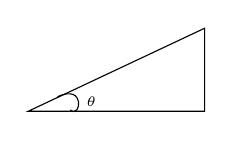
\begin{tikzpicture}[x=0.75pt,y=0.75pt,yscale=-1,xscale=1]
%uncomment if require: \path (0,300); %set diagram left start at 0, and has height of 300

%Shape: Right Triangle [id:dp7115443128693997] 
\draw   (255,114) -- (170,154) -- (255,154) -- cycle ;
%Curve Lines [id:da7600903054423039] 
\draw    (184.2,147) .. controls (197.8,140.6) and (195.4,157.8) .. (190.2,153.4) ;

% Text Node
\draw (196.8,145.6) node [anchor=north west][inner sep=0.75pt]  [font=\tiny]  {$\theta $};


\end{tikzpicture}

\end{center}
\end{description}
\end{aun}

\begin{exx}
Find the antiderivative of:
\[
\int \frac{1}{x^2 \sqrt{x^2 + 4}} dx
\]
\end{exx}
\ans{ Following the second column of the table above gives us the substitution $x = 2 \tan \theta$, $dx = 2 \sec^2 \theta d \theta$:
We see that:
\[
\sqrt{x^2 + 4} = \lrb{4 (\underbrace{\tan^2 \theta + 1}_{\sec^2(\theta)})}^\frac12 = 2 \sec \theta
\]
When we make all of the necessary substitutions, we have:
\[
\int \frac{1}{x^2 \sqrt{x^2 + 4}} dx =  \int \frac{2 \sec^2 \theta d \theta}{(4 \tan^2 \theta) 2\sec\theta } = \frac14 \int \frac{\sec \theta d \theta}{\tan^2 \theta} = \frac14 \int \frac{\cos \theta}{\sin^2 \theta } d \theta 
\]
This is a $u$-substitution integral, which we can compute as:
\[
-\frac{1}{4\sin \theta} + C = -\frac14\csc \theta  + C = - \frac{\sqrt{x^2 + 4}}{4x} + C
\]
}

\problembox{Evaluate the following:
\begin{enumerate}
\item	$\dst \int \frac{x}{\sqrt{1+x^2}}dx$
\item $\dst \int \frac{\sqrt{x^2 - 1}}{x^4}dx$
\end{enumerate}
}
\ans{
The first is a second row integral, so make the substitution $x = \tan \theta$. This gives you, after some simplification:
\[
\int \frac{x}{\sqrt{1+x^2}}dx = \int \frac{\tan(\theta)}{\sec(\theta)}  \sec^2 (\theta) d \theta = \int \sec(\theta) \tan (\theta) d \theta = \sec \theta + C
\]
Reversing our substitution, we solve:
\[
\int \frac{x}{\sqrt{1+x^2}}dx = \sqrt{x^2 + 1} + C
\]
The second integral can be rewritten using the third column:
\[
\int \frac{\sqrt{x^2 - 1}}{x^4} = \int \frac{\tan \theta}{\sec^4 \theta} \sec \theta \tan \theta d \theta = \int \tan^2 \theta \cos^3 \theta d \theta = \int \sin^2 \theta \cos \theta d \theta  = \frac{u^3}{3} + C
\]
for the $u$-substitution $u = \sin \theta$. Going back through and reversing our substitutions, we have:
\[
\frac{\sin^3 \theta}{3} = \frac{\lrp{x^2 - 1}^{3/2}}{3 x^3} + C
\]
}

\problembox{Compute the following integral
\[
\int \frac{dx}{\sqrt{9x^2 - 36x + 37}}
\]}
\ans{To begin, let's study the polynomial inside the radical:
\[
9x^2 - 36x + 37 = 9 \lrp{x^2 - 4x + \frac{37}{9}}
\]
Completing the square of what's in the parenthesis, we see:
\[
9x^2 - 36x + 37 = 9 \lrp{x^2 - 4x + 4 - 4 + \frac{37}{9}} = 9 \lrp{(x- 2)^2 + \frac19} = 9(x-2)^2 + 1
\]
Now we can replace the integrand with some that looks a bit more tractable: 
\[
\int \frac{dx}{\sqrt{9x^2 - 36x + 37}} = \int \frac{dx}{\sqrt{9(x-2)^2 + 1}} = \int \frac{du}{\sqrt{3u^2 + 1}}
\]
when $u = x-2$ and $du = dx$. By the table above, we may make the substitution $3u = \tan \theta$:
\[
u = \frac13 \tan \theta \quad \quad du = \frac13 \sec^2 \theta d \theta  \quad \quad \sqrt{3u^2 + 1} = \sec \theta 
\]
Transform the integrand then into:
\[
\int \frac{\frac13 \sec^2 \theta d\theta}{\sec \theta} = \frac13 \int \sec \theta d \theta = \frac13 \ln \lrabs{\sec \theta + \tan \theta} + C
\]
From here, we can make substitutions based on the triangle our substitution implied:

\begin{center}
\tikzset{every picture/.style={line width=0.75pt}} %set default line width to 0.75pt        
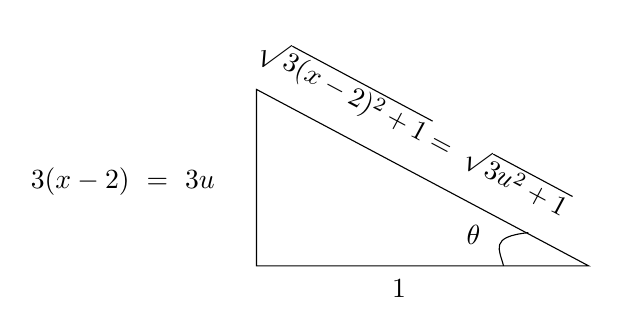
\begin{tikzpicture}[x=0.75pt,y=0.75pt,yscale=-1,xscale=1]
%uncomment if require: \path (0,300); %set diagram left start at 0, and has height of 300

%Shape: Right Triangle [id:dp6949691256097569] 
\draw   (259,98) -- (419,183) -- (259,183) -- cycle ;
%Curve Lines [id:da5515956445720602] 
\draw    (378,183) .. controls (376,175) and (371,169) .. (390,167) ;

% Text Node
\draw (359,162.4) node [anchor=north west][inner sep=0.75pt]    {$\theta $};
% Text Node
\draw (323,188.4) node [anchor=north west][inner sep=0.75pt]    {$1$};
% Text Node
\draw (149,134.4) node [anchor=north west][inner sep=0.75pt]    {$3( x-2) \ =\ 3u$};
% Text Node
\draw (264.4,68.51) node [anchor=north west][inner sep=0.75pt]  [rotate=-28.1]  {$\sqrt{3( x-2)^{2} +1} =\ \sqrt{3u^{2} +1}$};
\end{tikzpicture}
\end{center}
This gives us the final answer:
\[
\int \frac{dx}{\sqrt{9x^2 - 36x + 37}} = \ln{\sqrt{3(x-2)^2+1} + 3(x-2)}
\]
}

\end{document}